\section{Magnetic Fields}

\subsection{magnetism}

\subsubsection{magnets}\index{magnets}

magnetic effects are commonly seen in \emph{magnets}

a magnet creates a magnetic field that attracts or repels other magnets

\cmt polarity of magnets

a magnet has two poles, the \emph{north pole} and the \emph{south pole}

freely suspend a magnet, the north pole points towards earth's geographic north pole

when two magnets are brought near each other, like poles repel, and opposite poles attract

\cmt we use \keypoint{magnetic field lines}\index{field line!magnetic field line} to graphically represent how magnetic field permeate space

by convention, fields lines emerge from north pole and go into south pole

density of field lines shows strength of magnetic field

direction of field line tells how the north pole of a small compass will line up at that point

\cmt strength of the field is described by a quantity called \keypoint{magnetic flux density}, denoted by $B$

when we draw field lines, we are actually drawing the pattern of flux density $B$

the notion of flux density will be defined later in details in \S\ref{sec:magnetic_flux_density}

\example{magnetic field around a bar magnet}

\begin{center}
\begin{tikzpicture}[yscale=0.5,xscale=0.8]
\tikzstyle flines=[thick,blue,postaction={decorate},decoration={markings,mark=at position 0.56 with {\arrow{>}}}]
\draw [fill=blue!70] (-3,-1) rectangle (0,1);
\draw [fill=red] (0,-1) rectangle (3,1);
\node at (-1.5,0) {\Large \textcolor{white}{S}};
\node at (1.5,0) {\Large \textcolor{white}{N}};
\draw [flines] (3,0) -- (6.8,0);
\draw [flines] (-6.8,0) -- (-3,0);
\draw [flines] (3,0.2) [out=10,in=210] to (6.5,1.35);
\draw [flines] (3,-0.2) [out=-10,in=-210] to (6.5,-1.35);
\draw [flines] (3,0.5) [out=20,in=240] to (6,3.5);
\draw [flines] (3,-0.5) [out=-20,in=-240] to (6,-3.5);
\draw [flines] (-6.5,1.35) [out=-30,in=170] to (-3,0.2);
\draw [flines] (-6.5,-1.35) [out=30,in=190] to (-3,-0.2);
\draw [flines] (-6,3.5) [out=-60,in=160] to (-3,0.5);
\draw [flines] (-6,-3.5) [out=60,in=200] to (-3,-0.5);
\draw [flines] (3,0.9) [out=60,in=0] to (0,3.6) [out=180,in=120] to (-3,0.9);
\draw [flines] (3,-0.9) [out=-60,in=0] to (0,-3.6) [out=180,in=-120] to (-3,-0.9);
\draw [flines] (2.5,1) [out=150,in=30] to (-2.5,1);
\draw [flines] (2.5,-1) [out=-150,in=-30] to (-2.5,-1);
\end{tikzpicture}
\end{center}

\question{For two identical bar magnets placed side by side as shown, what does the magnetic field look like? Try sketching the magnetic field lines.}


\begin{center}
\begin{minipage}{0.48\linewidth}
\begin{center}
\begin{tikzpicture}[xscale=0.5,yscale=0.3]
\draw[white] (0,-6) -- (0,6);
\draw [fill=blue!70] (1,-1) rectangle (3,1);
\draw [fill=red] (3,-1) rectangle (5,1);
\draw [fill=blue!70] (-5,-1) rectangle (-3,1);
\draw [fill=red] (-3,-1) rectangle (-1,1);
\node at (2,0) {\textcolor{white}{S}};
\node at (4,0) {\textcolor{white}{N}};
\node at (-4,0) {\textcolor{white}{S}};
\node at (-2,0) {\textcolor{white}{N}};
\end{tikzpicture}

(a) two attracting bar magnets
\end{center}
\end{minipage}
\begin{minipage}{0.48\textwidth}
\begin{center}
\begin{tikzpicture}[xscale=0.5,yscale=0.3]
\draw[white] (0,-6) -- (0,6);
\draw [fill=red] (1,-1) rectangle (3,1);
\draw [fill=blue!70] (3,-1) rectangle (5,1);
\draw [fill=blue!70] (-5,-1) rectangle (-3,1);
\draw [fill=red] (-3,-1) rectangle (-1,1);
\node at (2,0) {\textcolor{white}{N}};
\node at (4,0) {\textcolor{white}{S}};
\node at (-4,0) {\textcolor{white}{S}};
\node at (-2,0) {\textcolor{white}{N}};
\end{tikzpicture}

(b) two repelling bar magnets
\end{center}
\end{minipage}
\end{center}

\subsubsection{magnetic field due to currents}
an electric current also induces a magnetic field around it

this was first discovered by Danish physicist \emph{Hans Christian Orsted} in 1820, when he noticed the turning of a compass needle placed next to a wire carrying current.

we will look into what happens when a current flows through a straight wire or a coil

\cmt pattern of the field can be determined using \keypoint{right-hand (grip) rule}\index{right-hand rule}\footnote{The awesome right-hand rule illustrations below are copied from the PSTricks web site: \url{http://tug.org/PSTricks/main.cgi?file=examples}. The credits for these figures are attributed to CTAN community member \emph{Thomas S\"{o}ll}.}

\begin{figure}[htp]
	\centering
\begin{minipage}{0.55\linewidth}
\begin{center}
\begin{tikzpicture}[scale=1.2,decoration={markings,mark=at position 0.7 with {\arrow{>}}}]
\foreach \l  in {0.2,0.4,0.7,1.1}
\draw[thick, blue, postaction={decorate}] (0,0) ellipse (\l*2.5 and \l);
\draw[white,fill] (-0.15,0) rectangle (0.15,1.2);
\draw [very thick, postaction={decorate}] (0,-2.4) -- (0,-1.2) (0,0) -- (0,2) node[below right]{current};
\draw [very thick, dashed] (0,-1.1) -- (0,-0.1);
\draw (-1.8,-1.3) node {field};
\end{tikzpicture}
\end{center}
\end{minipage}
\begin{minipage}{0.35\linewidth}
\begin{center}
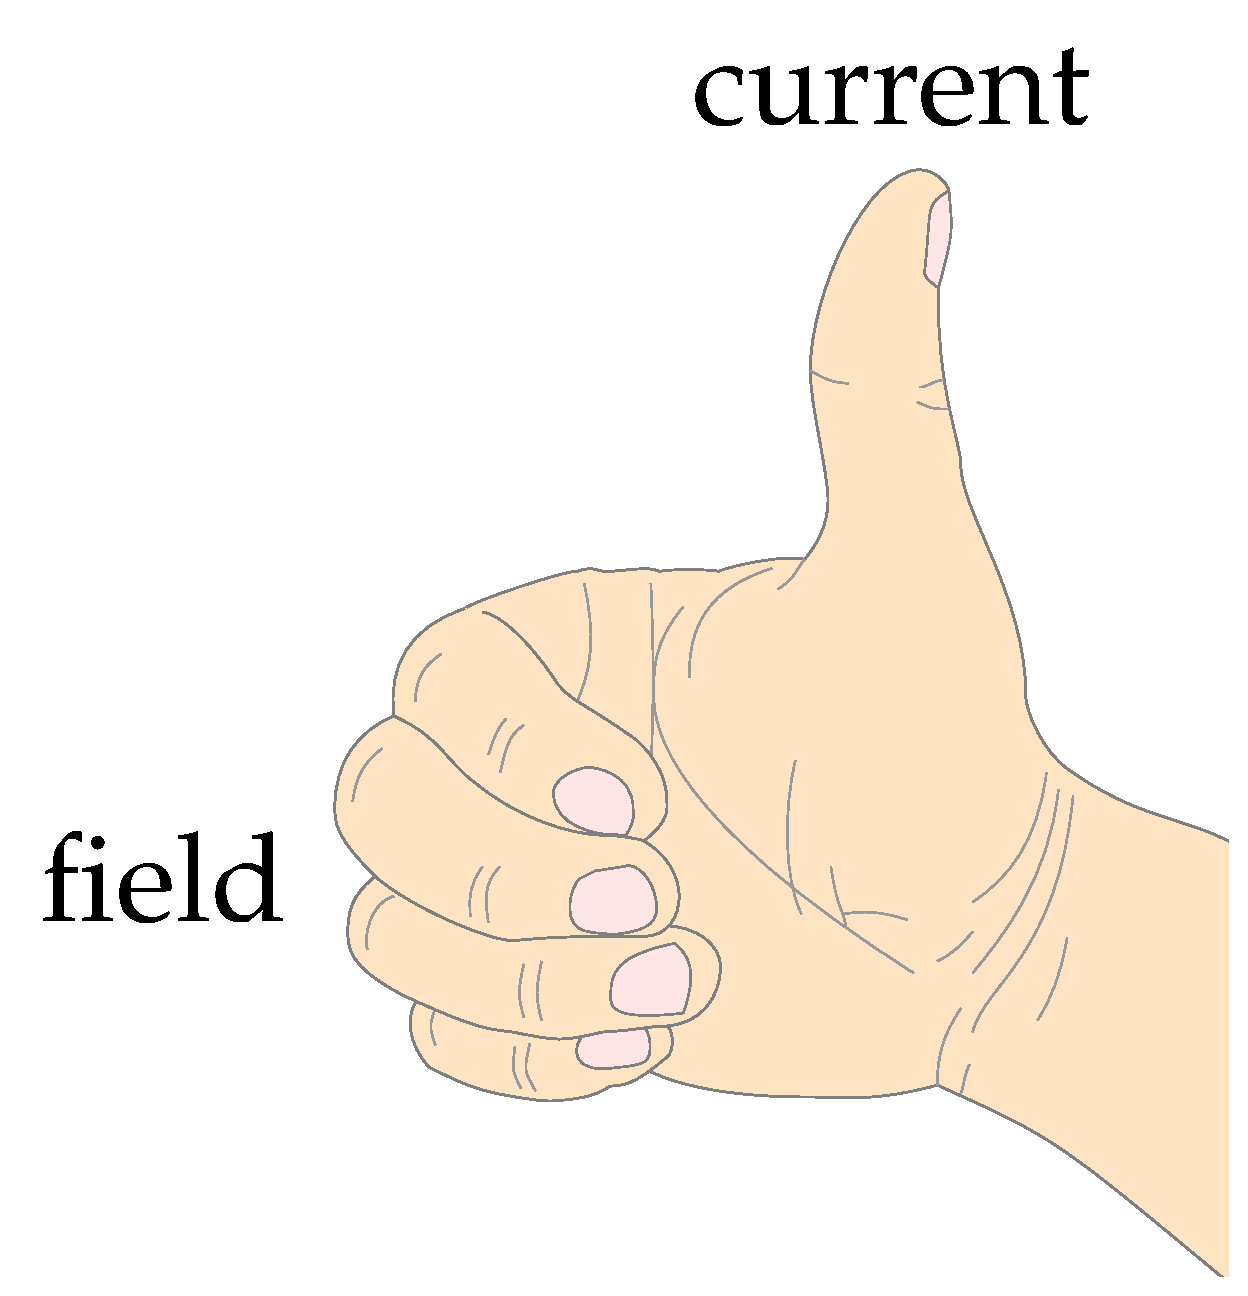
\includegraphics[height=108pt]{right-hand-straight.pdf}
\end{center}
\end{minipage}

\vspace{0.8em} field due to a long straight current-carrying wire
\end{figure}

\begin{figure}[htp]
	\centering
\begin{minipage}{0.3\linewidth}
	\begin{center}
		\begin{tikzpicture}[scale=0.9,decoration={markings,mark=at position 0.75 with {\arrow{>}}}]
		\draw[very thick, postaction={decorate}] (0,0) ellipse (1.0 and 0.5);
		\draw (1.6,-0.5) node {current};
		\draw[white,fill] (-0.15,0.4) rectangle (0.15,0.6);
		\draw[white,fill] (-0.6,0.3) rectangle (-0.4,0.5);
		\draw[white,fill] (0.6,0.3) rectangle (0.4,0.5);
		\draw [very thick, blue, postaction={decorate}] (0,-2.4) -- (0,-0.7) (0,0) -- (0,2);
		\draw [very thick, blue, postaction={decorate}] (0.96,-2.4) [out=120,in=-84] to (0.54,-0.7) (0.5,0) [out=90,in=-110] to (0.9,2);
		\draw [very thick, blue, postaction={decorate}] (-0.96,-2.4) [out=60,in=-96] to (-0.54,-0.7) (-0.5,0) [out=90,in=-70] to (-0.9,2);
		\draw [very thick, blue, dashed] (0,-0.7) -- (0,-0.1);
		\draw [very thick, blue, dashed] (0.54,-0.7) [out=96,in=-90] to (0.5,0);
		\draw [very thick, blue, dashed] (-0.54,-0.7) [out=84,in=-90] to (-0.5,0);
		\draw (1.4,1.5) node {field};
		\end{tikzpicture}
	\end{center}
\end{minipage}
\begin{minipage}{0.4\linewidth}
	\begin{center}
		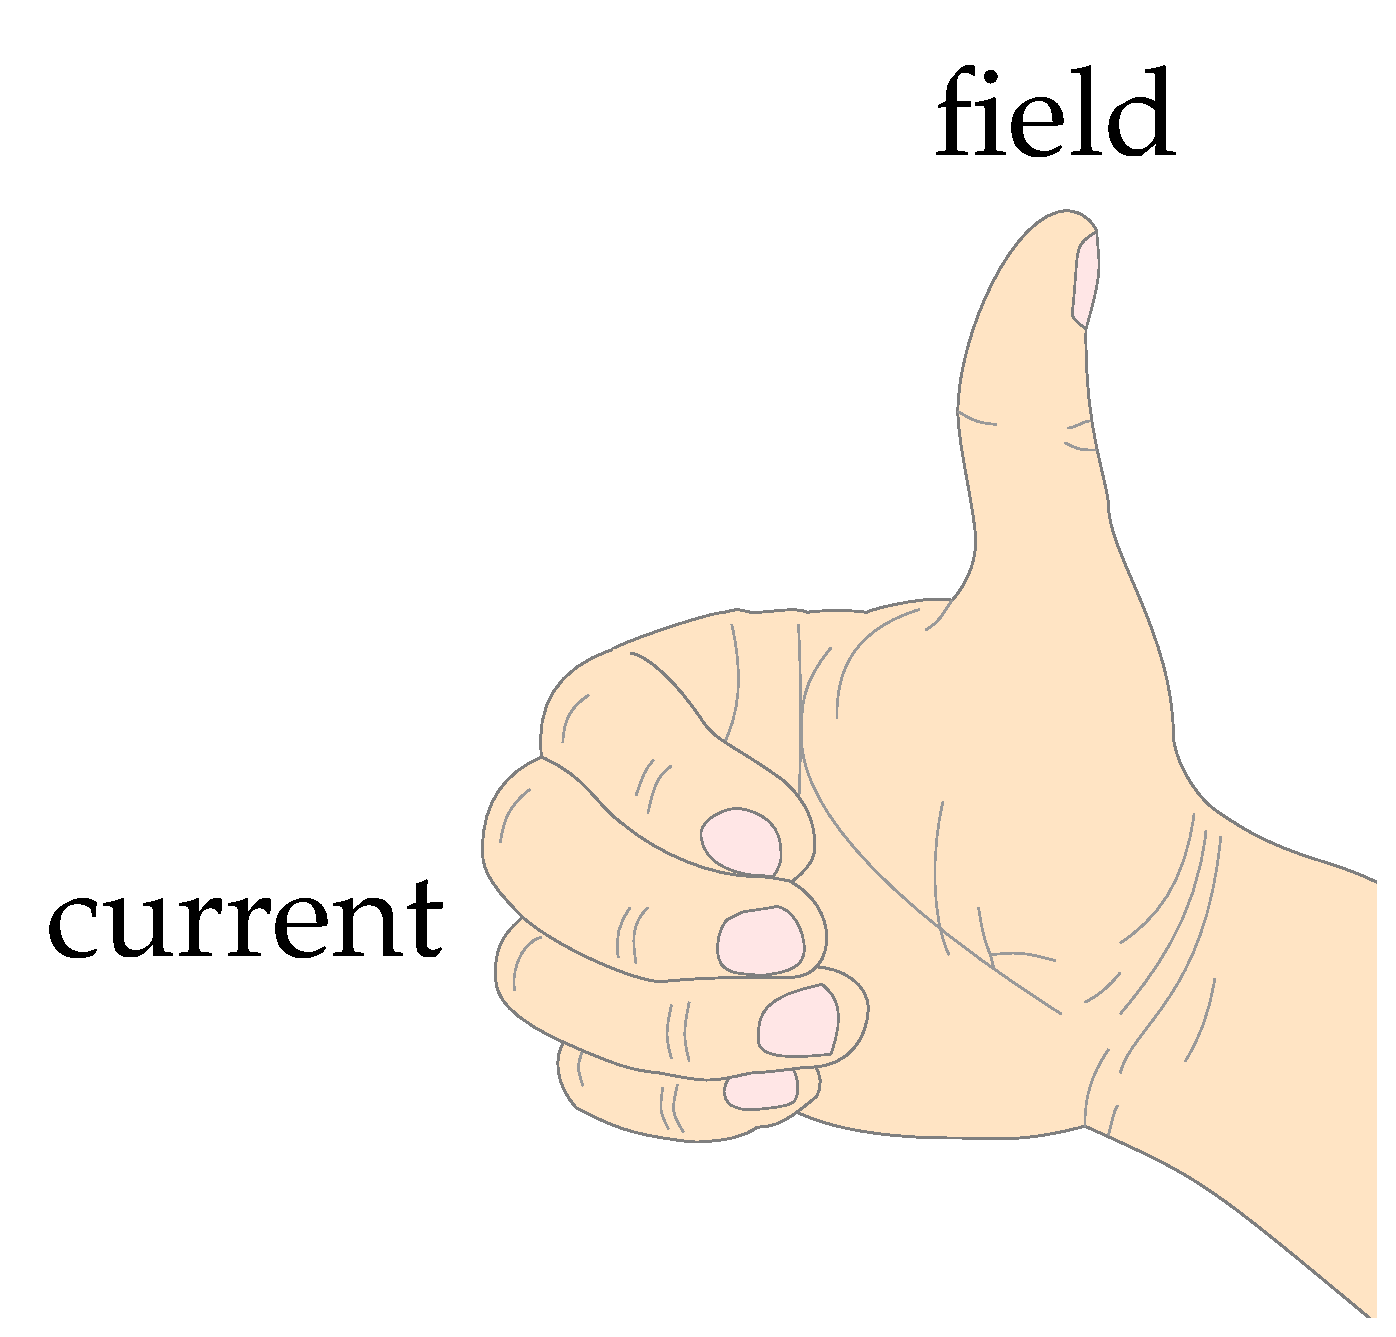
\includegraphics[height=120pt]{right-hand-circular.pdf}
	\end{center}
\end{minipage}

\vspace{0.8em} field due to a circulating current
\end{figure}

\cmt strength of the field is proportional to the current: $B \propto I$

for both straight wires
\footnote{The magnetic flux density generated by a current flowing in an infinitely long wire in free space is given by: $\boxed{B=\frac{\mu_0 I}{2\pi r}}$, $I$ is the electric current, $r$ is the perpendicular distance from the current, and $\mu_0 = 4\pi \times 10^{-7} \text{ T m A}^{-1}$ is a fundamental physical constant called the \emph{vacuum permeability}\index{permeability of free space}. ($\star$)}
 and coils\footnote{The magnetic flux density at the centre of a current-carrying coil in free space is given by: $\boxed{B=\frac{\mu_0 NI}{L}}$, where $N$ is the number of turns, $I$ is the electric current flowing through the coil, $L$ is the length of coil, and $\mu_0$ is the vacuum permeability. ($\star$)}
 , greater current means stronger field
 
\cmt magnetic field can be increased with \emph{soft iron}

\emph{ferromagnetic materials} (iron, cobalt, nickel, etc.) can attract magnetic field lines, so they can greatly increases strength of the field\footnote{If the straight wire is immersed in a material with \emph{relative permeability} $\mu_r$, then the field becomes: $B=\frac{\mu_0 \mu_r I}{2\pi r}$. Similarly, if a material with relative permeability $\mu_r$ is present, then the magnetic flux density inside a coil becomes: $B=\frac{\mu_0 \mu_r NI}{L}$. A good magnetic material (high permeability material), such as iron, has large $\mu_r$, and therefore can greatly intensify the magnetic field. ($\star$)}

\subsubsection{solenoids \& electromagnets}

strength and polarity of the field due to a coil can be changed easily by tuning currents, so coils are widely used to create magnetic fields where needed

a current-carrying coil is also called a \keypoint{solenoid}\index{solenoid}

\begin{figure}[htp]
	\centering
	\begin{minipage}{0.65\linewidth}
		\begin{center}
			\begin{tikzpicture}[yscale=0.6,xscale=0.7]
			\tikzstyle flines=[thick,blue,postaction={decorate},decoration={markings,mark=at position 0.56 with {\arrow{>}}}] % field line style
			\tikzstyle ct=[very thick,postaction={decorate},decoration={markings,mark=at position 0.54 with {\arrow{>}}}] % coil style
			
			\draw [flines] (3,0) -- (6.8,0);
			\draw [flines] (3,0.2) [out=10,in=210] to (6.5,1.35);
			\draw [flines] (3,-0.2) [out=-10,in=-210] to (6.5,-1.35);
			\draw [flines] (3,0.5) [out=20,in=240] to (6,3.5);
			\draw [flines] (3,-0.5) [out=-20,in=-240] to (6,-3.5);
			
			\draw [flines] (3,0.9) [out=60,in=0] to (0,3.6) [out=180,in=120] to (-3,0.9);
			\draw [flines] (3,-0.9) [out=-60,in=0] to (0,-3.6) [out=180,in=-120] to (-3,-0.9);
			\draw [flines] (2.5,1) [out=150,in=30] to (-2.5,1);
			\draw [flines] (2.5,-1) [out=-150,in=-30] to (-2.5,-1);
			\draw[ct] (-2.6,-3.5) --++ (0,3);
			
			\draw[thick,fill=white] (3,0) ellipse (0.35 and 1);
			\draw[thick,white,fill] (-3,-1) rectangle (3,1);
			\draw[thick,fill=white] (-3,0) ellipse (0.35 and 1);
			\draw[thick] (-3,-1) -- (3,-1);
			\draw[thick] (-3,1) -- (3,1);
			\foreach \k in {-2.5,-2.0,...,2.1} {\draw[ct] (\k,1) [out=60, in=-120] to (\k+0.4,-1);}
			\draw[very thick] (2.5,1) [out=60, in=-120] to (2.9,-1);
			\draw[white,fill] (2.6,-.978) rectangle (2.8,0);
			\draw[white,fill] (2.7,-1.1) rectangle (2.9,-1.022);
			\draw[very thick] (2.7,0.1) -- (2.7,-1);
			\draw[ct] (2.7,-1) --++ (0,-2.5);
			
			\draw [flines] (-6.8,0) -- (-3,0);
			\draw [flines] (-6.5,1.35) [out=-30,in=170] to (-3,0.2);
			\draw [flines] (-6.5,-1.35) [out=30,in=190] to (-3,-0.2);
			\draw [flines] (-6,3.5) [out=-60,in=160] to (-3,0.5);
			\draw [flines] (-6,-3.5) [out=60,in=200] to (-3,-0.5);
			
			\draw (2.8,-2.1) --++ (1.2,-0.8) node[below]{current};
			\node at (5.8,2) {field};
			\node at (3.6,1.4) {N};
			\node at (-3.6,1.4) {S};
			\end{tikzpicture}
		\end{center}
	\end{minipage}
	\begin{minipage}{0.3\linewidth}
		\begin{center}
		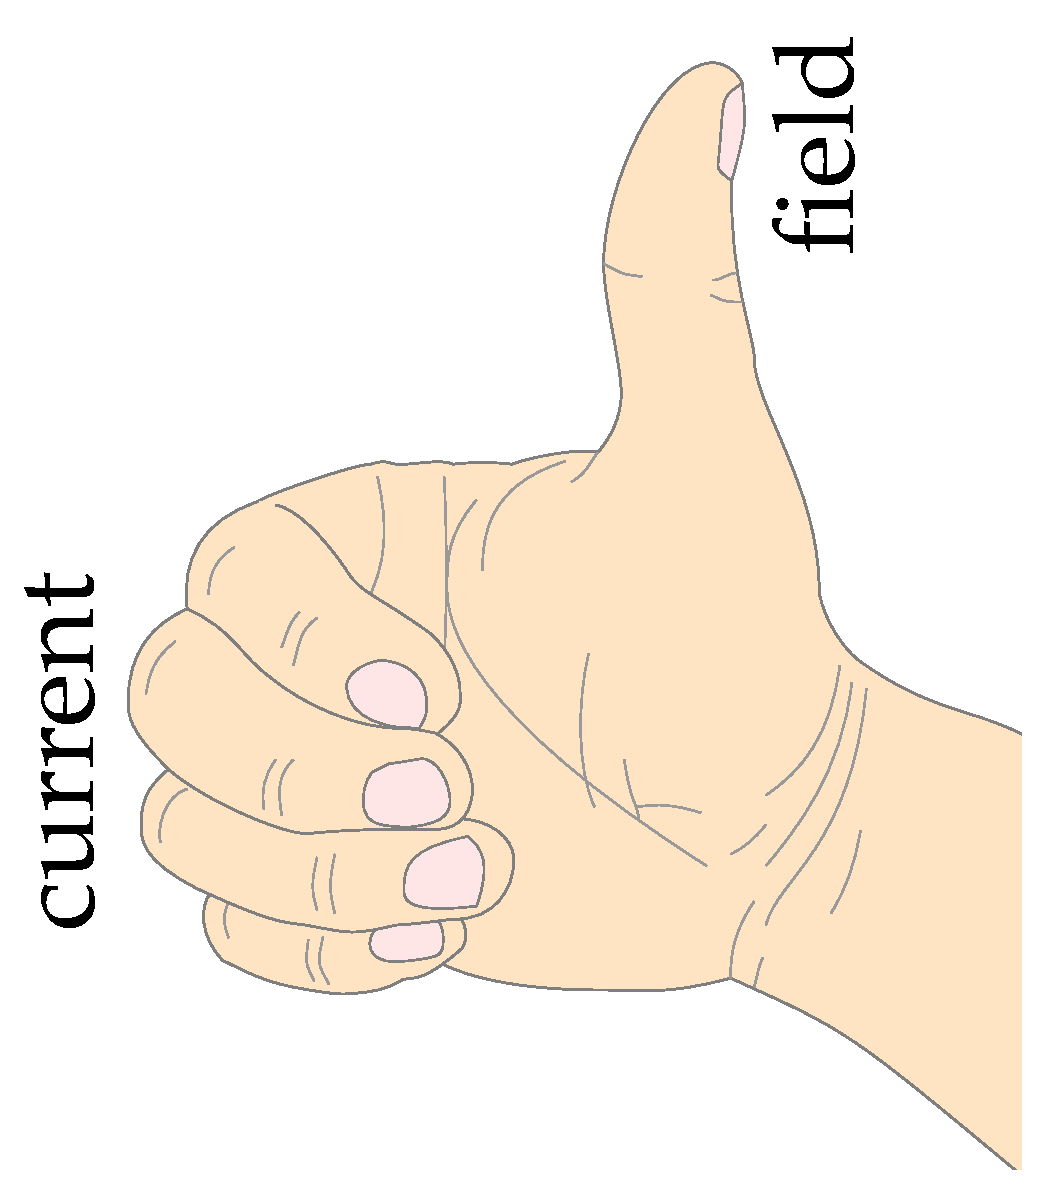
\includegraphics[height=120pt,angle=-90]{right-hand-coil.pdf}
		\end{center}
	\end{minipage}
	
	\vspace{0.8em} magnetic field around a solenoid
\end{figure}

\cmt a solenoid generates a magnetic field similar to that of a bar magnet

useful to talk about the north and south poles of a solenoid

\cmt direction of magnetic field in a solenoid is given by the \keypoint{right-hand (grip) rule}\index{right-hand rule}

%\cmt a solenoid produces a \emph{uniform} magnetic field in its centre and near its poles

\cmt magnetic field produced by a solenoid can be controlled

current $I\up \ra $ stronger field, also number of turns $N\up\ra $ stronger field

\cmt inserting an \emph{iron core} inside greatly strengthens the field, this makes an \emph{electromagnet}

\question{Describe the magnetic field due to an alternating current through a solenoid.}


\subsection{magnetic force on current-carrying conductor}

\subsubsection{magnetic force on current-carrying conductor}

a current-carrying wire produces its own magnetic field, when it is surrounded by an external magnetic field, the two fields would interact $\Rightarrow$ a \keypoint{magnetic force}\index{magnetic field!magnetic force} on the conductor

\begin{wrapfigure}{r}{0.4\textwidth}
	\vspace*{-16pt}
	\centering
	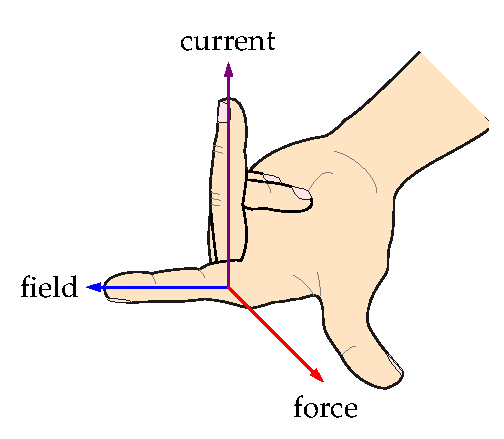
\includegraphics[height=135pt]{left-hand.pdf}
	
	Fleming's left-hand rule
	\vspace*{-16pt}
\end{wrapfigure}

\cmt direction of magnetic force on current can be worked out with \keypoint{Fleming's left-hand rule}\index{left-hand rule}\footnote{Figure credit again goes to \emph{Thomas S\"{o}ll} from the CTAN community.}

\cmt magnitude of magnetic force: $\boxed{F=BIL\sin\theta}$

$B$ is the magnetic flux density to be specified later

$I$ is the current, $\theta$ is the angle between $B$ and $I$

\cmt when $B \perp I$, magnetic force $F=BIL$

when $B \parallelslant I$, there is no magnetic force

when $B$ forms angle $\theta$ with $I$, only the \emph{perpendicular component} contributes to the force, giving rise to the $\sin\theta$ factor in the formula

\cmt magnetic force is perpendicular to both $B$ and $I$
\footnote{Vector form of the formula: $\vec{F} = l\vec{I} \times \vec{B}$. ($\star$)}

\example{Determine the direction of the magnetic force acting. Check yourself.}
\begin{center}
	\begin{minipage}[b]{0.32\textwidth}
		\centering
		\begin{tikzpicture}[scale=0.45]
		\foreach \y in {-2,2} \foreach \x in {-2,2}
		\node at (\x,\y) {\large\textcolor{blue}{$\times$}};
		%magnetic fields
		\draw[ultra thick,->] (-3.5,0) -- (2,0) node[below]{\textcolor{black}{$I$}} ;
		\draw[ultra thick] (2,0) -- (3.5,0); %currents
		\draw[red,very thick,->] (0,0) -- (0,2.4) node[right]{$F$};
		\node[blue,above right] at (2,2) {$B$};
		\end{tikzpicture}
		
		(a)
	\end{minipage}
	\begin{minipage}[b]{0.32\textwidth}
		\centering
		\begin{tikzpicture}[scale=0.4]
		\foreach \y in {-2,2} \foreach \x in {-2,2}
		\draw[blue,fill] (\x,\y) circle(0.1);
		%magnetic fields
		\draw[ultra thick,->] (0,-3.5) -- (0,2) node[right]{\textcolor{black}{$I$}} ;
		\draw[ultra thick] (0,2) -- (0,3.5); %currents
		\draw[red,very thick,->] (0,0) -- (2.4,0) node[below]{$F$};
		\node[blue,above right] at (2,2) {$B$};
		\end{tikzpicture}
		
		(b)
	\end{minipage}
\begin{minipage}[b]{0.32\textwidth}
	\centering
	\begin{tikzpicture}[scale=0.64,decoration={markings,mark=at position 0.84 with {\arrow{>}}}]
	\foreach \y in {-2,2}
	{
		\draw[blue,thick,postaction={decorate}] (-3,\y) -- (3,\y);
	}
	%magnetic fields
	\node[blue] at (3.4,1) {$B$};
	\draw [very thick, postaction={decorate}] (-2,0) -- ++(0:4) node[right] {$I$};
	\node[red,below] at (0,-0.3) {$F=0$};
	\end{tikzpicture}
	
	(c)
\end{minipage}
\end{center}


\subsubsection{magnetic flux density} \label{sec:magnetic_flux_density}

rewrite $F=BIL\sin\theta$ as $B = \frac{F}{IL\sin\theta}$,we can now give a formal definition for flux density $B$:

\begin{ilight}
	\keypoint{magnetic flux density}\index{magnetic field!magnetic flux density} $B$ at a point is defined as the force acted per unit length on a conductor carrying a unit current at right angle to the magnetic field
\end{ilight}

\cmt flux density describes the strength of a magnetic field\footnote{Magnetic field strength is a different quantity, defined by $H=\frac{B}{\mu}$, with $\mu=\mu_0\mu_r$ being the \emph{magnetic permeability} of material. The naming of field strength $H$ and flux density $B$ are due to historical reasons.}

\cmt $B$ is measured in \keypoint{tesla}\index{tesla} (T)\footnote{Telsa is a very large unit. For example, the strength of a typical refrigerator magnet is of about $10^{-3} \text{ T}$, even the very strong superconducting coils used in MRI are of around $1\sim3 \text{ T}$.}: $[B]=\text{T}$, $1 \text{ T} = 1 \text{ N}\cdot\text{A}^{-1}\cdot\text{m}^{-1}$

\begin{ilight}
	if a wire of 1 m normal to the magnetic field that carries a current of $1\text{ A}$ experiences a force of $1\text{ N}$, then the magnetic flux density is $1\text{ T}$
\end{ilight}

\cmt $B$ is a \emph{vector} quantity, with both magnitude and direction


\example{A wire of 0.80 m carrying a current of 5.0 A is lying at right angles to a magnetic field, it experiences a force of 0.60 N, what is the flux density?}
	
\sol $B=\frac{F}{IL} = \frac{0.60}{5.0\times0.80} = 0.15 \text{ T} \quad $ (a field of over 0.1 T is actually quite strong!) \eoe


\newpage
\example{Torque on a rectangular metal frame in uniform magnetic field}

\begin{wrapfigure}{l}{0.36\textwidth}
	\vspace*{-12pt}
	\centering
	\begin{tikzpicture}[scale=0.96,decoration={markings,mark=at position 0.75 with {\arrow{>}}}]
	\draw[very thick, postaction={decorate}] (0,0) -- (0,3);
	\draw[very thick, postaction={decorate}] (0,3) -- (2,3);
	\draw[very thick, postaction={decorate}] (2,3) -- (2,0);
	\draw[very thick,postaction={decorate}] (0.8,-1.4) -- (0.8,0) -- (0,0);
	\draw[very thick,postaction={decorate}] (2,0) -- (1.2,0) --++ (0,-1.4);
	\foreach \y in {0.5,2.5} {
		\draw[blue,thick,->] (-1,\y) -- (3,\y);
	}
	\node[above,blue] at (3,2.5) {$B$};
	\node[below left] at (0,0) {$P$};
	\node[above left] at (0,3) {$Q$};
	\node[above right] at (2,3) {$R$};
	\node[below right] at (2,0) {$S$};
	\node[right] at (2,1) {$I$};
	\node[right,red] at (2.1,1.5) {$F$};
	\node[left,red] at (-0.1,1.5) {$F$};
	
	\draw[thick,<->] (-1.5,0) --++ (0,3) node[left, midway]{$L$};
	\draw[thick,<->] (0,3.6) --++ (2,0) node[midway,above]{$d$};
	
	\draw[white,fill] (2,1.5) circle (0.18);
	\draw[white,fill] (0,1.5) circle (0.18);
	\draw[red,thick] (2,1.5) circle (0.18);
	\draw[red,thick,fill] (2,1.5) circle (0.06) (0.6,1.3) node[above right]{$I$};
	\draw[red,thick] (0,1.5) circle (0.18);
	\draw[red,very thick] (-0.1,1.4) -- (0.1,1.6) (-0.1,1.6) -- (0.1,1.4);
	\end{tikzpicture}
	\vspace*{-8pt}
\end{wrapfigure}

a rectangular frame lies in parallel with the field

$QR, PS \parallelslant B$, so no force acting on these two sides

$PQ, RS \perp B$, so there is magnetic force $F=BIL$

using left-hand rule, we find $F_{PQ}$ acts into the paper, $F_{RS}$ acts out of the paper

this is a pair of equal but opposite forces

they produce a torque about central axis of frame: $\tau=Fd=BILd$, causing the frame to rotate\footnote{This effect allows engineers to build \emph{electric motors}, such as those in electric vehicles, washing machines, blenders, etc.}\eoe

\question{If the plane of the rectangular frame is at right angle to the magnetic field, describe the magnetic forces acting on each side and hence state what happens to the frame.}

\begin{wrapfigure}{r}{0.35\textwidth}
	\vspace*{-12pt}
	\centering
	\begin{tikzpicture}[scale=0.75]
	\draw[ultra thick] (-2.5,0) rectangle (2.5,4);
	\draw[ultra thick] (-1.5,1) rectangle (1.5,4);
	\draw[ultra thick, white] (-1.47,4) -- (1.47,4);
	\node at (0,4) {\large $\otimes$};
	\node[above] at (0,4.1) {$I$};
	\node at (2,3.6) {$N$};
	\node at (-2,3.6) {$S$};
	\draw[ultra thick] (-3,-2) rectangle (3,-0.1);
	\draw[thick] (-1.5,-1.6) rectangle (1.5,-0.5);
	\node at (0,-1.1) {\large 500.0 g};
	\end{tikzpicture}
	\vspace*{-12pt}
\end{wrapfigure}

\example{A U-shaped magnet is placed on a balance with a wire suspended above it as shown. Magnetic flux density between the poles is about 0.50 T. The part of the wire that is in the field is of length 8.0 cm. The balance initially shows a reading of 500.0 g. When a current of 10 A flowing into the paper is switched on, what is the new reading on the balance?}\label{ex-mag-balance}

\sol use left-hand rule, force on wire acts upwards

from \emph{Newton's third law}, reaction force on magnet acts downwards

so there will be an increase in the balance reading

magnitude of the force: $F=BIl = 0.50 \times 10 \times 8.0\times10^{-2} = 0.40 \text{ N}$

change in the mass reading: $\Delta m = \frac{F}{g} = \frac{0.40}{9.81} \approx 0.0407 \text{ kg} \approx 40.7 \text{ g}$

new reading on balance: $m_\text{new} = 500.0 + 40.7 = 540.7 \text{ g}$ \eoe

\question{If the current in Example \ref{ex-mag-balance} is replaced by a current of 6.0 A flowing out of the plane of the paper. What is the reading on the balance?}

\subsubsection*{force between long straight current-carrying wires}

\begin{center}
\begin{minipage}{0.3\linewidth}
\begin{center}
\begin{tikzpicture}[scale=0.84,decoration={markings,mark=at position 0.6 with {\arrow{>}}}]
\draw[ultra thick, postaction={decorate}] (-1.2,0) node[left]{$I_1$} (-1.2,-2) -- (-1.2,2);
\draw[ultra thick, postaction={decorate}] (1.2,0) node[right]{$I_2$} (1.2,-2) -- (1.2,2);
\end{tikzpicture}
\end{center}
\end{minipage}
\begin{minipage}{0.35\linewidth}
\begin{center}
\begin{tikzpicture}[scale=0.56,decoration={markings,mark=at position 0.4 with {\arrow{>}}}]
\draw[black,thick] (0,0) circle (0.25);
\draw[black,thick,fill] (0,0) circle (0.06) (0,0.2) node[above]{$I_1$};
\draw[black,thick] (3,0) circle (0.25);
\draw[black,thick,fill] (3,0) circle (0.06) (3,0.2) node[above left]{$I_2$};
\draw[thick, blue, postaction={decorate}] (4:3) arc [radius=3, start angle=5, end angle=356];
\draw[blue] (144:3.6) node{$B_1$};
\draw[red,thick,->] (3,0) -- (1.2,0) node[below]{$F_{21}$};
\end{tikzpicture}
\end{center}
\end{minipage}
\begin{minipage}{0.3\linewidth}
\begin{center}
\begin{tikzpicture}[scale=0.84,decoration={markings,mark=at position 0.6 with {\arrow{>}}}]
\draw[ultra thick, postaction={decorate}] (-1.2,0) node[left]{$I_1$} (-1.2,-2) -- (-1.2,2);
\draw[ultra thick, postaction={decorate}] (1.2,0) node[right]{$I_2$} (1.2,-2) -- (1.2,2);
\draw[red,thick,->] (1.2,0) -- (0.1,0) node[below right]{$F_{21}$};
\draw[red,thick,->] (-1.2,0) -- (-0.1,0) node[below left]{$F_{12}$};
\end{tikzpicture}
\end{center}
\end{minipage}
\end{center}

if we have two straight parallel wires carrying currents in the same direction

force acting on $I_2$ is due to magnetic field $B_1$ generated by $I_1$

from top view, $I_1$ creates a counter-clockwise $B_1$, so $I_2$ experiences an upward field

using left-hand rule, force acting on $I_2$ by $I_1$, denoted $F_{21}$\footnote{$F_{AB}$ denotes the force acted on object $A$ by object $B$.}, points to the left

since $F_{21}$ and $F_{12}$ are a pair of action-reaction, so $F_{12}$ points to the right


\begin{center}
\begin{minipage}{0.3\linewidth}
\begin{center}
\begin{tikzpicture}[scale=0.84,decoration={markings,mark=at position 0.6 with {\arrow{>}}}]
\draw[ultra thick, postaction={decorate}] (-1.2,0) node[left]{$I_1$} (-1.2,-2) -- (-1.2,2);
\draw[ultra thick, postaction={decorate}] (1.2,0) node[right]{$I_2$} (1.2,2) -- (1.2,-2);
\end{tikzpicture}
\end{center}
\end{minipage}
\begin{minipage}{0.35\linewidth}
\begin{center}
\begin{tikzpicture}[scale=0.56,decoration={markings,mark=at position 0.4 with {\arrow{>}}}]
\draw[black,thick] (0,0) circle (0.25);
\draw[black,thick,fill] (0,0) circle (0.05) (0,0.2) node[above]{$I_1$};
\draw[black,thick] (3,0) circle (0.25);
\draw[black,thick] (3,0.2) node[above left]{$I_2$};
\draw[black,thick] (3.13,0.13) -- (2.87,-0.13) (3.13,-0.13) -- (2.87,0.13);
\draw[thick, blue, postaction={decorate}] (4:3) arc [radius=3, start angle=5, end angle=356];
\draw[blue] (144:3.6) node{$B_1$};
\draw[red,thick,->] (3,0) -- (4.8,0) node[below]{$F_{21}$};
\end{tikzpicture}
\end{center}
\end{minipage}
\begin{minipage}{0.3\linewidth}
\begin{center}
\begin{tikzpicture}[scale=0.84,decoration={markings,mark=at position 0.6 with {\arrow{>}}}]
\draw[ultra thick, postaction={decorate}] (-1.2,0) node[right]{$I_1$} (-1.2,-2) -- (-1.2,2);
\draw[ultra thick, postaction={decorate}] (1.2,0) node[left]{$I_2$} (1.2,2) -- (1.2,-2);
\draw[red,thick,->] (1.2,0) -- (2.2,0) node[below left]{$F_{21}$};
\draw[red,thick,->] (-1.2,0) -- (-2.2,0) node[below right]{$F_{12}$};
\end{tikzpicture}
\end{center}
\end{minipage}
\end{center}

similar discussions apply for $I_1$ and $I_2$ flowing in opposite directions (left as exercise)

hence we come to an conclusion: \emph{parallel currents attract, and anti-parallel currents repel}\footnote{The S.I. unit for current, ampere, is defined using two long wires parallel to each other carrying the same current in the same direction. If the wires are separated by 1 m and the magnetic force experienced per metre is $2.0\times10^{-7}$ N, then the current is of 1 A.}

\question{A coil of wire of several loops is suspended from a fixed point. When an electric current is switched on in the coil, state and explain the change in the separation between the loops.}

\question{Two long parallel wires carry currents of $I_1=$3.0 A and $I_2=$5.0 A in the same direction as shown. The flux density at a point at perpendicular distance $r$ from a straight long wire carrying current $I$ is given by $B=\frac{\mu_0 I}{2\pi r}$.}\label{q-pwires}



\begin{figure}[htp]
\centering
\begin{tikzpicture}[scale=1.2,decoration={markings,mark=at position 0.65 with {\arrow{>}}}]
\draw[very thick, postaction={decorate}] (0,0) --++ (0,4) node[pos=0.55, left]{$I_1$};
\draw[very thick, postaction={decorate}] (3,0) --++ (0,4) node[pos=0.55, left]{$I_2$};
\draw[gray,dashed,thick] (-2.5,1) --++ (1.5,2) --++ (6.5,0) --++ (-1.5,-2) --++ (-6.5,0); 
\end{tikzpicture}
\end{figure}

\begin{compactenum}
\item[(a)] Draw at least three lines to show the magnetic field due to $I_1$.

\item[(b)] State and explain the direction of force acting on $I_2$.

\item[(c)] Given that $I_1$ and $I_2$ are separated by 4.0 cm, what is flux density due to $I_1$ at $I_2$?

\item[(d)]  What is the magnetic force per unit length acting on $I_2$?

\item[(e)] What is the magnitude and the direction of the force per unit length acting on $I_1$?
	
\end{compactenum}

\question{If the current in one of the two wires in Question \ref{q-pwires} is replaced by an alternating current, then the two wires should begin to vibrate. However, the wires are not observed to move. Make some reasonable estimates and explain why the vibration is not observed.}







\subsection{magnetic force on charged particles}

electric currents are formed by moving charges, since current-carrying wires in a magnetic field experience force, charged particle moving in magnetic field should also experience force

\subsubsection{magnetic force on charged particles}

starting from $F=BIl\sin\theta$, let's substitute $I=nAqv \RA F=B(nAqv)l\sin\theta$

notice $n$ is the number density of charged particles, so $nAl$ together gives the total number

if we look at the force acting on \emph{one} charged particle, then $nAl=1$, so: $F=Bqv\sin\theta$

\cmt magnitude of magnetic force on charged particle: $\boxed{F=Bqv\sin\theta}$ 

$B$ is magnetic flux density, $q$ is electric charge of the particle, $v$ is its velocity

$\theta$ refers to the angle between $B$ and $v$

\begin{wrapfigure}{r}{0.36\textwidth}
	\vspace*{-16pt}
	\centering
	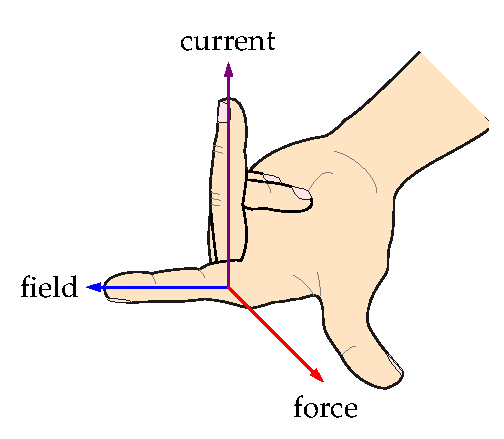
\includegraphics[height=135pt]{left-hand.pdf}
	
	Fleming's left-hand rule
	\vspace*{-16pt}
\end{wrapfigure}

\cmt direction of magnetic force can be determined using \emph{Fleming's left-hand rule}\index{left-hand rule}

for $+q$, current in same direction as $v$

for $-q$, current in opposite direction as $v$

\cmt force depends on \emph{perpendicular component} of $B$

if $v \perp B$, magnetic force $F=Bqv$

if $v \parallelslant B$, there is no magnetic force

when particle moves at angle $\theta$ to $B$, contribution to the force only comes from the \emph{perpendicular component}, giving rise to the $\sin\theta$ factor

\cmt magnetic force always perpendicular to both velocity $v$ and magnetic field $B$\footnote{Vector form of the formula: $\vec{F} = q\vec{v} \times \vec{B}$. ($\star$)}

\example{Use the left-hand rule to find the direction of the magnetic forces acting on the following moving charges. Check yourself.}
\begin{center}
	\begin{minipage}[b]{0.45\textwidth}
		\centering
		\begin{tikzpicture}[scale=1]
		\draw[blue,dashed] (-2.7,-2.7) rectangle (2.7,2.7);
		\foreach \y in {-2,0,2} \foreach \x in {-2,0,2}
		\node at (\x,\y) {\large\textcolor{blue}{$\times$}};
		%magnetic fields
		\draw[purple,very thick,->] (-1.1,-1.2) --++ (1.5,0) node[midway,above]{$v$};
		\draw[red,very thick,->] (-1.1,-1.2) --++ (0,1.8) node[left]{$F$};
		\shade [ball color = orange] (-1.1,-1.2) circle (0.15);
		\node[below] at (-1.1,-1.4) {$+q$};
		\draw[purple,very thick,->] (1.2,1.2) --++ (0,-1.5) node[midway,right]{$v$};
		\draw[red,very thick,->] (1.2,1.2) --++ (-1.8,0) node[above]{$F$};
		\shade [ball color = green] (1.2,1.2) circle (0.15);
		\node[above] at (1.2,1.4) {$-q$};
		\node[blue,above right] at (2,2) {$B$};
		\end{tikzpicture}
		
		(a)
	\end{minipage}
	\begin{minipage}[b]{0.45\textwidth}
		\centering
		\begin{tikzpicture}[scale=1]
		\draw[blue,dashed] (-2.7,-2.7) rectangle (2.7,2.7);
		\foreach \y in {-2,0,2} \foreach \x in {-2,0,2}
		\draw[blue,fill] (\x,\y) circle(0.05);
		%magnetic fields
		\draw[purple,very thick,->] (-0.6,-1.2) --++ (110:1.4) node[midway,above right]{$v$};
		\draw[red,very thick,->] (-0.6,-1.2) --++ (20:1.8) node[below]{$F$};
		\shade [ball color = orange] (-0.6,-1.2) circle (0.15);
		\node[below] at (-0.6,-1.4) {proton};
		\draw[purple,very thick,->] (1,0.5) --++ (70:1.2) node[midway,right]{$v$};
		\draw[red,very thick,->] (1,0.5) --++ (160:1.8) node[above]{$F$};
		\shade [ball color = green] (1,0.5) circle (0.15);
		\node[below] at (1,0.3) {electron};
		\node[blue,above right] at (2,2) {$B$};
		\end{tikzpicture}
		
		(b)
	\end{minipage}
\end{center}

\subsubsection*{charged particles in electric \& magnetic fields}

in either electric field or magnetic field, charged particle may experience a force\footnote{The combination of electric and magnetic force on the charge due to electromagnetic fields is called the \emph{Lorentz force}\index{Lorentz force}: $\vec{F} = q(\vec{E} + \vec{v}\times \vec{B})$. If you have a good knowledge in maths, everything we cover in this section can be recovered from this vector equation. ($\star$)}

in this section, we will compare the difference between electric field and magnetic field

\begin{center}
	{%\renewcommand{\arraystretch}{1.2}
		\begin{tabular}{|D{0.22\textwidth}|D{0.36\textwidth}|D{0.3\textwidth}|}
			
			\hline
			& electric field & magnetic field \\ \hline
			
			strength of the field & electric field strength $E$ & magnetic flux density $B$ \\ \hline
			
			magnitude of force & $F_E = Eq$ & $F_B=Bqv\sin\theta$ \\ \hline
			
			whether force depends on velocity & no dependence, acts equally on stationary or moving charges & depend on perpendicular component of velocity \\ \hline
			
			\multirow{2}{*}{direction of force} & $F_E \parallelslant E$ &  $F_B \perp B$ and $F_B \perp v$ \\
			
			& same as/opposite to $E$ for $+q$/$-q$ & use left-hand rule\\ \hline
			
			effect of force on motion of particle & can change both magnitude and direction of velocity & only changes direction of velocity, cannot change magnitude of velocity \\ \hline
			
			work done by force & work can be done, can define notions of potential and P.E. & magnetic force does no work for charged particles\\ \hline
			
	\end{tabular}}
\end{center}



\subsubsection{charged particle in uniform magnetic fields}

suppose a charged particle is moving at right angle to a uniform magnetic field

\begin{figure}[htp]
	\centering
	\begin{tikzpicture}[scale=0.75]
			\draw[blue, dashed] (-4,-4) rectangle (4,4);
			\foreach \x in {-3,0,3}{
				\foreach \y in {-3,0,3}{
					\node[draw,circle,blue,inner sep=0.8pt,fill] at (\x,\y) {};  }}
			\node[blue] at (-2.5,2.5) {$B$};
			\draw[thick,dotted] (0,0) circle [radius=2.5];
			\foreach \s in {80,200,310}
			{
				\draw [purple, thick, ->] (\s:2.5) -- ++(\s-90:2);
				\draw [purple] (\s-35:3.5) node{$v$};
				\draw [red, thick, ->] (\s:2.5) -- (\s:0.8);
				\draw [red] (\s+25:1) node{$F$};
				\shade [ball color = yellow] (\s:2.5) circle (0.25) node{\footnotesize$+$};
			}
	\end{tikzpicture}
\end{figure}

magnetic force $F_B$ always at right angle to motion, so $F_B$ keeps changing direction of velocity

uniform field means a constant force, so $F_B$ deflects the particle at the same rate

the particle should describe a \emph{circular} path!

\begin{ilight}
	for a charged particle moving in a uniform magnetic field, \emph{magnetic force provides centripetal force for circular motion}: $\boxed{Bqv = \frac{mv^2}{r}}$, or $\boxed{Bqv = m \omega^2 r}$
\end{ilight}

\cmt can solve for radius of the orbiting particles: $r=\frac{mv}{Bq}$

\begin{compactenum}

\item[-] $v\up \Rightarrow r\up$, faster particles take larger circles
	
\item[-] $B\up \Rightarrow r\down$, stronger magnetic field, larger centripetal force, smaller circles
	
\item[-] $m\up \Rightarrow r\up$, larger mass, larger inertia, so larger circles

\end{compactenum}
	
\cmt radius of curvature relates to charge-to-mass ratio (also called \emph{specific charge}\index{specific charge}) of the particle

rearrange the equation we have $\frac{q}{m}=\frac{v}{Br}$, which can be computed using experimental data

\example{An $\alpha$-particle travelling at $2.5\times10^4 \mps$ enters a region of uniform magnetic field. The field has flux density of 5.4 mT and is normal to direction of particle's velocity. What is the radius of $\alpha$-particle's path?}

\sol radius of circular arc: $r=\frac{mv}{Bq} = \frac{4\times 1.66\times10^{-27}\times2.5\times10^4}{5.4\times10^{-3}\times2\times1.60\times10^{-19}} \approx 0.096 \text{ m} \approx 9.6 \text{ cm}$ \eoe

\question{For an $\alpha$-particle and a $\beta$-particle entering the same uniform magnetic field at a same speed, compare the radius of their paths.}

\question{For a charged particle undergoing circular motion in a uniform magnetic field, show that its angular velocity is independent of the radius of its path.}

\question{If a charged particle enters a uniform magnetic field at an angle $\theta \neq 90^\circ$, state and explain the path of this particle. (Hint: think about components of its velocity.)}
	
\subsubsection{mass spectrometer}

a \keypoint{mass spectrometer}\index{mass spectrometer} is a device to measure the charge-to-mass ratio of charged particles

\begin{figure}[htp]
	\centering
	\begin{tikzpicture}[scale=0.72,decoration={markings,mark=at position 0.7 with {\arrow{>}}}]
	% electric fields
	\draw[orange,dashed,fill=orange!20] (-8,1.5) rectangle (-4,-1.5);
	\draw[ultra thick] (-8,-1.5) --++ (0,3);
	\draw[ultra thick] (-4,-1.5) --++ (0,1.3) (-4,1.5) --++ (0,-1.3);
	\draw (-6,-1) --++ (-1.2,-1.5) node[twoline,below]{accelerating voltage\\supply of p.d. $V$};
	% magnetic field
	\draw[dashed,blue,fill=blue!10] (0,1) rectangle (5,-9);
	\node[blue] at (3.6,-0.4){$B$};
%	\foreach \y in {0.167,-1.5,-3.167,-4.833,-6.5,-8.167} \foreach \x in {0.833,2.5,4.167}
%	\node[blue] at (\x,\y) {$\times$};
	\draw (4.5,-0.5) --++ (1.2,1.2) node[twoline,right]{uniform magnetic\\field region};
	% paths of particle beam
	\draw [thick,purple,postaction={decorate}] (0,0) arc(90:-90:4);
	\draw [thick,purple,postaction={decorate}] (0,0) arc(90:-90:3);
	\draw [thick,purple,postaction={decorate}] (-8,0) -- (-4,0);
	\draw [thick,purple,postaction={decorate}] (-4,0) -- (0,0);
	\node[purple,above] at (-2,0) {$v$};
	\shade [ball color = green] (-7,0) circle (0.2);
	\shade [ball color = green] (-3,0) circle (0.2);
	\draw[<->] (-0.3,0) --++ (0,-8) node[midway,left]{$d=2r$};
	% detectors
	\draw[gray!50,fill] (-1,-5) rectangle(-0.7,-9);
	\draw (-0.85,-6.5) --++ (-1,1) node[left,twoline]{particle\\detector};
	\end{tikzpicture}
	
	mass spectrometer
\end{figure}

charged particles accelerated through an electric field: $\frac{1}{2}mv^2 = qV$

they then enter a uniform magnetic field: $Bqv = \frac{mv^2}{r} \ra v=\frac{Bqr}{m}$ $\quad$

eliminating $v$: $v^2 = \frac{2qV}{m} = \frac{B^2 q^2 r^2}{m^2} \ra \frac{q}{m} = \frac{2V}{B^2 r^2}$

we can measure $V$, $B$, $r$ in practice, so the charge-to-mass ratio $\frac{q}{m}$ is worked out

since different particles usually have different values of $\frac{q}{m}$, so this technique is widely used to identify unknown particles

\question{In the figure above, two paths of deflected particles are shown. Give reasons why the radius of the circular path can be different.}

\question{If the particles sent into the mass spectrometer are positively-charged, in which direction should the magnetic field be applied?}

\question{A particle carrying a charge of $+e$ enters a uniform magnetic field of $8.8$ mT at right angles with an initial speed of $1.4\times10^5 \text{ m s}^{-1}$. It describes a semi-circle with diameter of 66 cm. (a) Find the mass of the particle. (b) Suggest possible composition of this particle.}

\subsubsection{cyclotron}\index{cyclotron}

a \keypoint{cyclotron} is a type of \emph{particle accelerator}

\begin{figure}[htp]
	\centering
	\begin{tikzpicture}[decoration={markings,mark=at position 0.6 with {\arrow{>}}}, scale=1.2]
	\def\gap{0.6}
	% magnetic fields
	\draw[thick, dashed, blue, fill=blue!10] (-2.6,0) arc(180:25:2.73) [out=-25, in = 100] to (10:3.2) arc(10:0:3.2) --cycle;
	\draw[thick, dashed, blue, fill=blue!10] (-2.6,-\gap) arc(180:360:2.9) -- cycle;
	% electric field
	\draw[thick, dashed, blue, fill=orange!20] (-2.6,0) rectangle (3.2,-\gap);
	% semi-circular paths
	\draw[thick, postaction={decorate}] (1,0) arc(0:180:1);
	\draw[thick, postaction={decorate}] (-1,-\gap) arc(180:360:1.414);
	\draw[thick, postaction={decorate}] (1.818,0) arc(0:180:1.732);
	\draw[thick, postaction={decorate}] (-1.636,-\gap) arc(180:360:2);
	\draw[thick, postaction={decorate}] (2.364,0) arc(0:180:2.236);
	\draw[thick, postaction={decorate}] (-2.108,-\gap) arc(180:360:2.449);
	% accelerating paths
	\foreach \x in {1.818,2.364,2.791} \draw[thick, postaction={decorate}] (\x,-\gap) --++ (0,\gap);
	\foreach \x in {-1, -1.636, -2.108} \draw[thick, postaction={decorate}] (\x, 0) --++ (0,-\gap);
	\draw[thick, postaction={decorate}] (2.791,0) --++(0,3);
	\draw[thick] (1,-\gap/2) --++(0,\gap/2);
	% proton source
	\draw[fill] (1,-\gap/2) circle(0.1);
	% nodes
	\draw (0.207, -\gap) ++ (200:2.6) -- (-4,0.8) (160:2.3) -- (-4,1) node[left,twoline]{magnetic field\\into the paper};
	\draw (-2.4,-\gap/2) -- (-3.6,-1) node[left,twoline]{high-frequency\\alternating\\electric field};
	\draw (1,-\gap/2) -- (3.2,-2.8) node[right,twoline]{proton\\source};
	\draw (2.791,2.2) -- (1,3.5) node[above, twoline]{outgoing beam of\\high-speed protons};
	\end{tikzpicture}
	
	cyclotron
\end{figure}

the idea is to makes use of magnetic force to guide moving charges into a spiral path between accelerations by an electric field

as the particle enters and leaves the region of electric field, it gains extra energy of $qV$

it then follows a semi-circular path under magnetic force and re-enters the electric field

polarity of the electric field is reversed so the particle continues to accelerate across the gap

energy of particle increases by $qV$, it then moves in a larger semi-circle in magnetic field

repeat this process, the particle leaves the exit port with very high speed



\cmt cyclotron frequency

for charged particles circulating in a uniform magnetic field: $Bqv=m\omega^2 r$

time to complete one full turn is: $T=\frac{2\pi r}{v} = \frac{2\pi}{v}\times\frac{mv}{Bq}\ra T=\frac{2\pi m}{Bq}$

this shows the period is independent of radius of the circular path!

if an alternating voltage is applied at frequency $f=\frac{Bq}{2\pi m}$, particles can be accelerated continuously at just the right time when they cross the gap

this frequency is known as the \emph{cyclotron frequency}

\question{Protons are accelerated in a cyclotron where the uniform magnetic field region has a flux density of 1.5 T and the voltage between the gap is 20 kV. (a) Find the frequency of the voltage supply needed. (b) Find the number of circles the protons must make in order to gain an energy of 10 MeV.}


\subsubsection{velocity selector}

\keypoint{velocity selector}\index{velocity selector} is a device to produce a beam of charged particles all with same speed $v$

\begin{figure}[htp]
	\centering
	\begin{tikzpicture}[xscale=0.9,yscale=0.8]
	\foreach \x in {-2,2}
	\foreach \y in {-1.5,1.5}
	\node[blue] at (\x,\y) {$\times$};
	\foreach \x in {-3,-1,...,3}
	\draw[orange,thick,->] (\x,3) -- (\x,-3);
	\node[blue] at (-2,2.1) {$B$};
	\node[orange] at (3.5,-2) {$E$};
	\draw[ultra thick] (-4,3) -- (4,3);
	\draw[ultra thick] (-4,-3) -- (4,-3);
	\draw[ultra thick] (0,-4.5) node[right]{$-$} -- (0,-3) (0,3) -- (0,4.5) node[right]{$+$};
	\draw [fill] (-4.2,0.2) rectangle (-4,3.6);
	\draw [fill] (-4.2,-0.2) rectangle (-4,-3.6);
	\draw [fill] (4.2,0.2) rectangle (4,3.6);
	\draw [fill] (4.2,-0.2) rectangle (4,-3.6);
	\shade [ball color = green] (-6.5,0) circle (0.1);
	\node[below,twoline] at (-6.5,-0.2) {electron\\beam};
	\draw[purple,thick,->] (-6.2,0) -- (-5,0) node[above,midway]{$v$};
	\draw[purple,thick,->] (-5,0) -- (6,0) node[above]{$v=\frac{E}{B}$};
	\draw[purple] (-4,0) [out=0,in=210] to (4,2);
	\node[purple,right] at (4.2,2) {$v<\frac{E}{B}$};
	\draw[purple] (-4,0) [out=0,in=160] to (4,-1.5);
	\node[purple,right] at (4.2,-1.5) {$v>\frac{E}{B}$};
	\shade [ball color = green] (0,0) circle (0.1);
	\draw[red,thick,->] (0,0.2) -- (0,2) node[above]{\textcolor{black}{$F_E=Eq$}};
	\draw[red,thick,->] (0,-0.2) -- (0,-2) node[below]{\textcolor{black}{$F_B=Bqv$}};
	
	\end{tikzpicture}
	
	velocity selector
\end{figure}

let's consider a beam of electrons passing through a region where both uniform electric field and magnetic field are applied, electrons at desired speed $v$ are \emph{undeflected}

no net force acting on these electrons, so equilibrium between electric and magnetic force

{

\centering

$F_E = F_B \RA Eq = Bqv \RA \boxed{v=\frac{E}{B}}$

}

for particles entering the same region with higher speed, $F_B>F_E$, they deflect upwards

for particles entering the same region with lower speed, $F_B<F_E$, they deflect downwards

\question{If electrons at speed $v$ are undeflected when they pass through the velocity selector, what about a beam of $\alpha$-particles entering the same region at the same speed $v$?}

\question{A uniform magnetic field with flux density $6.0\times10^{-2} \text{ T}$ is applied out of the plane of the paper. A beam of protons are travelling into this region at a speed of $3.5\times10^4 \text{m s}^{-1}$. (a) In which direction do the protons deflect? (b) A uniform electric field is now applied in the same region so that the protons become undeviated. What is the strength and the direction of this electric field?}


\subsection{Hall effect}
when an electric current passes through a conductor surrounded by an external magnetic field perpendicular to the current, a transverse potential difference is produced

this phenomenon is known as the \keypoint{Hall effect}\index{Hall effect} (discovered by American physicist \emph{Edwin Hall} in 1879), the voltage difference is called the \keypoint{Hall voltage}

\vspace*{\baselineskip}

suppose magnetic field goes upward, current flows to the right (see figure), then charge carriers (assumed to be electrons for now) experience a magnetic force pointing out of paper

\begin{figure}[ht]
	\centering
	\begin{tikzpicture}[scale=1]
	\draw[thick] (-6,.5) -- ++(3,0); % current in
	\draw[thick,fill=gray!30] (-4,-1) -- ++(0,1) -- ++(3,2) -- ++(4,0) -- ++(0,-1)  -- ++(-3,-2) -- cycle;
	\draw[thick] (-4,0) -- (0,0) -- (3,2) (0,0) -- (0,-1); %conductor
	\draw[blue,thick,->] (-.5,-2.5) -- (-.5,-1) (-.5,1) -- ++(0,2) node[right]{$B$}; %magnetic fields
	\draw[thick,->] (1.5,.5) -- ++(3,0) node[above]{$I$}; % current out
	\shade [ball color = green] (-1.1,1) circle (0.12);
	\draw[thick,purple,->] (-1.1,1) -- ++(-1,0) node[above right]{$v$};
	\draw[thick,red,->] (-1.1,1) -- ++(-1,-.667) node[left]{$F_B$};
	\end{tikzpicture}
\end{figure}

this magnetic force causes a build-up of extra charge on front side of conductor, which produces an internal electric field $E$ inside conductor, i.e., a potential difference $V_H$ is formed

\begin{figure}[ht]
	\centering
	\begin{tikzpicture}[scale=1]
	\draw[thick] (-6,.5) -- ++(3,0); % current in
	\draw[thick,fill=gray!30] (-4,-1) -- ++(0,1) -- ++(3,2) -- ++(4,0) -- ++(0,-1)  -- ++(-3,-2) -- cycle;
	\draw[thick] (-4,0) -- (0,0) -- (3,2) (0,0) -- (0,-1); %conductor
	\draw[blue,thick,->] (-.5,-2.5) -- (-.5,-1) (-.5,1) -- ++(0,2) node[right]{$B$}; %magnetic fields
	\draw[thick,->] (1.5,.5) -- ++(3,0) node[above]{$I$}; % current out
	\shade [ball color = green] (-1.1,1) circle (0.12);
	\draw[thick,purple,->] (-1.1,1) -- ++(-1,0) node[above right]{$v$};
	\draw[thick,red,->] (-1.1,1) -- ++(-1,-.667) node[left]{$F_B$};
	\draw[thick,violet,->] (-1.1,1) -- ++(1,.667) node[right]{$F_E$};
	\foreach \ball in {-3.5,-2.5,-1.5,-0.5}{
		\shade [ball color = green] (\ball,-0.5) circle (0.12);
		\draw[thick] (\ball-0.05,-0.5) --++ (0.1,0);
	}
	\draw[thick,olive,<->] (-4.8,0) -- ++(3,2) node[midway,above left]{$V_H$};
	\draw[thick,olive,<-] (-0.8,.3) node[left]{$E$} -- ++(2.1,1.4);
	\draw[thick,<->] (.5,-1.35) -- ++(3,2) node[midway, below right]{$d$};
	\draw[thick,<->] (3.5,1) -- ++(0,1) node[midway, right]{$t$};
	\end{tikzpicture}
\end{figure}

as charge carriers accumulate on one side, Hall voltage opposes further migration of charges

steady $V_H$ is established when magnetic force and electric force are balanced: $Eq = Bqv$

\begin{compactenum}
	\item[-] strength of internal electric field is related to Hall voltage: $E=\frac{V_H}{d}$
	
	where $d$ is width of the conductor
	
	\item[-] drift velocity $v$ of particles is related to current $I$: $I=nAqv$
	
	where $A$ is cross section of conductor and $n$ is number density of charge carriers
\end{compactenum}


we now have: $\frac{V_H}{d}q = Bq \frac{I}{nAq} \ra V_H = \frac{BId}{nAq}$

note that cross section $A=dt$, where $t$ is thickness of conductor as shown

we therefore obtain an useful expression for Hall voltage: $ V_H = \frac{BId}{n(td)q} \ra \boxed{V_H = \frac{BI}{ntq}}$ 

\cmt to produce noticeable $V_H$, we want smaller $n$ and smaller $t$

\begin{compactenum}
	\item[-] $n\downarrow \ra$ few free charge carriers $\ra$ \emph{semi-conductors} are preferable

	\item[-] $t\downarrow \ra$ small thickness $\ra$ \emph{thin slice} of component is preferable

\end{compactenum}

\cmt polarity of $V_H$ is determined by nature of charge carries
	
charge carriers can be \emph{free electrons} (negatively charged) or \emph{holes} (positively charged)
	
then Hall voltage induced would have opposite polarity

\cmt if current $I$ forms angle $\theta$ with flux density $B$, again only perpendicular component matters

expression for Hall voltage becomes: $V_H = \frac{BI}{ntq}\sin\theta$
	
\cmt apply a fixed current in a conductor, $V_H$ is proportional to $B$
	
so magnetic flux density can be calculated once we find $V_H$
	
one can make use of Hall effect to build a \emph{Hall probe}, a device used to measure flux density $B$

when using a Hall probe, one should rotate and record the greatest voltage reading to ensure the current applied is at right angle to the external magnetic field

\question{Why is it difficult to detect Hall voltage in a thin slice of copper?}

\question{A Hall probe is placed near to one end of a strong magnet. State and explain the variation in the Hall voltage as the probe is rotated for one complete revolution.}
	
